% Options for packages loaded elsewhere
\PassOptionsToPackage{unicode}{hyperref}
\PassOptionsToPackage{hyphens}{url}
%
\documentclass[
  english,
  ,man,floatsintext]{apa6}
\usepackage{lmodern}
\usepackage{amssymb,amsmath}
\usepackage{ifxetex,ifluatex}
\ifnum 0\ifxetex 1\fi\ifluatex 1\fi=0 % if pdftex
  \usepackage[T1]{fontenc}
  \usepackage[utf8]{inputenc}
  \usepackage{textcomp} % provide euro and other symbols
\else % if luatex or xetex
  \usepackage{unicode-math}
  \defaultfontfeatures{Scale=MatchLowercase}
  \defaultfontfeatures[\rmfamily]{Ligatures=TeX,Scale=1}
\fi
% Use upquote if available, for straight quotes in verbatim environments
\IfFileExists{upquote.sty}{\usepackage{upquote}}{}
\IfFileExists{microtype.sty}{% use microtype if available
  \usepackage[]{microtype}
  \UseMicrotypeSet[protrusion]{basicmath} % disable protrusion for tt fonts
}{}
\makeatletter
\@ifundefined{KOMAClassName}{% if non-KOMA class
  \IfFileExists{parskip.sty}{%
    \usepackage{parskip}
  }{% else
    \setlength{\parindent}{0pt}
    \setlength{\parskip}{6pt plus 2pt minus 1pt}}
}{% if KOMA class
  \KOMAoptions{parskip=half}}
\makeatother
\usepackage{xcolor}
\IfFileExists{xurl.sty}{\usepackage{xurl}}{} % add URL line breaks if available
\IfFileExists{bookmark.sty}{\usepackage{bookmark}}{\usepackage{hyperref}}
\hypersetup{
  pdftitle={What might books be teaching young children about gender?},
  pdfauthor={XXX, XX, XXX, XXX, \& XXX},
  pdflang={en-EN},
  pdfkeywords={reading, gender, language development},
  hidelinks,
  pdfcreator={LaTeX via pandoc}}
\urlstyle{same} % disable monospaced font for URLs
\usepackage{graphicx,grffile}
\makeatletter
\def\maxwidth{\ifdim\Gin@nat@width>\linewidth\linewidth\else\Gin@nat@width\fi}
\def\maxheight{\ifdim\Gin@nat@height>\textheight\textheight\else\Gin@nat@height\fi}
\makeatother
% Scale images if necessary, so that they will not overflow the page
% margins by default, and it is still possible to overwrite the defaults
% using explicit options in \includegraphics[width, height, ...]{}
\setkeys{Gin}{width=\maxwidth,height=\maxheight,keepaspectratio}
% Set default figure placement to htbp
\makeatletter
\def\fps@figure{htbp}
\makeatother
\setlength{\emergencystretch}{3em} % prevent overfull lines
\providecommand{\tightlist}{%
  \setlength{\itemsep}{0pt}\setlength{\parskip}{0pt}}
\setcounter{secnumdepth}{-\maxdimen} % remove section numbering
\shorttitle{Gender in children's books}
\affiliation{
\vspace{0.5cm}
\textsuperscript{1} XXX\\\textsuperscript{2} XXX}
\keywords{reading, gender, language development\newline\indent Word count: XXX (excluding methods and results)}
\usepackage{csquotes}
\usepackage{upgreek}
\captionsetup{font=singlespacing,justification=justified}

\usepackage{longtable}
\usepackage{lscape}
\usepackage{multirow}
\usepackage{tabularx}
\usepackage[flushleft]{threeparttable}
\usepackage{threeparttablex}

\newenvironment{lltable}{\begin{landscape}\begin{center}\begin{ThreePartTable}}{\end{ThreePartTable}\end{center}\end{landscape}}

\makeatletter
\newcommand\LastLTentrywidth{1em}
\newlength\longtablewidth
\setlength{\longtablewidth}{1in}
\newcommand{\getlongtablewidth}{\begingroup \ifcsname LT@\roman{LT@tables}\endcsname \global\longtablewidth=0pt \renewcommand{\LT@entry}[2]{\global\advance\longtablewidth by ##2\relax\gdef\LastLTentrywidth{##2}}\@nameuse{LT@\roman{LT@tables}} \fi \endgroup}
\usepackage{setspace}
\usepackage{float}
\usepackage{graphicx}
\usepackage{tabu}
\usepackage{makecell}
\AtBeginEnvironment{tabular}{\singlespacing}
\usepackage{pbox}
\usepackage{hyphsubst}
\floatplacement{figure}{t!}
\raggedbottom
\renewcommand{\topfraction}{1}
\renewcommand{\bottomfraction}{1}
\renewcommand{\textfraction}{.1}
\renewcommand{\floatpagefraction}{1}
\ifxetex
  % Load polyglossia as late as possible: uses bidi with RTL langages (e.g. Hebrew, Arabic)
  \usepackage{polyglossia}
  \setmainlanguage[]{english}
\else
  \usepackage[shorthands=off,main=english]{babel}
\fi

\title{What might books be teaching young children about gender?}
\author{XXX\textsuperscript{1}, XX\textsuperscript{2}, XXX\textsuperscript{2}, XXX\textsuperscript{2}, \& XXX\textsuperscript{2}}
\date{}

\authornote{

Correspondence concerning this article should be addressed to XXX, XXX. E-mail: XXX}

\abstract{
We investigated how gender is represented in children's books using a 200,000 word corpus comprising 247 popular, contemporary books for young children (0-5 years). Using human judgments and word co-occurrence data, we quantified the gender biases of words within the corpus and within individual books. We find that children's books contain large numbers of words that adults judge as gendered. Semantic analyses based on co-occurrence data yielded word clusters related to gender stereotypes (e.g., feminine: emotions; masculine: tools). Co-occurrence data also indicate that books instantiate gender stereotypes found in other research (e.g., girls are better at reading and boys at math). Finally, we used large-scale data to estimate the gender distribution of the audience for individual books, and find that children tend to be exposed to gender stereotypes for their own gender. Together the data suggest that children's books may be an early source of gender stereotypes.

STATMENT OF RELEVANCE: Gender stereotypes such as that girls are better at reading and boys are better at math have origins in early childhood. We examined the extent to which popular children's books may expose young 0-5 year old children to information about gender stereotypes. Our data suggest that children's books have rich information about gender stereotypes, and that some of these stereotypes are more strongly represented in children's books than in adult fiction. These findings suggest that popular children's books may be unintentionally teaching young children about gender stereotypes.


}

\begin{document}
\maketitle

Many gender stereotypes held by adults have origins in early childhood. Beginning in their second year, children already exhibit knowledge of behaviors that are stereotypically feminine (e.g., vacuuming), masculine (e.g., building), and neutral (e.g., sleeping; Poulin-Dubois, Serbin, Eichstedt, Sen, \& Beissel, 2002). By age three, children distinguish individuals by gender, race, and age (Shutts, Banaji, \& Spelke, 2010). By age five, children have developed \enquote{a constellation of stereotypes about gender (often amusing and incorrect) that they apply to themselves and others} (Martin \& Ruble, 2004). For example, preschoolers act in accordance with the stereotype that girls are better at reading while boys are better at math (Cvencek et al., 2011b), and that girls are less likely than boys to be \enquote{very, very smart} (Bian, Leslie, \& Cimpian, 2017).

The \emph{sources} of this knowledge are less well understood. Certainly, some of what children know about gender characteristics comes from their own and observed interactions with adults (Hilliard \& Liben, 2010). Toys and activities are often gender stereotyped in home, day care, and preschool social settings (Weisgram, Fulcher, \& Dinella, 2014). Another source of information is language. Children commonly receive feedback from adults about gender-normative activities, e.g., girls more often receive adult linguistic feedback for dress and helping behaviors, whereas boys receive comments on their size and physical skills (Chick, Heilman-Houser, \& Hunter, 2002), and children are surprisingly sensitive to seemingly small differences in linguistic descriptions of gender-related information. For example, Cimpian \& Markman (2011) found that when a novel game was introduced to children using a generic subject (\enquote{Girls are really good at a game called \enquote{gorp}}) they were more likely to associate it with a gender than when the game was introduced with a specific subject (\enquote{There is a girl who is good at\ldots{}}). This sensitivity may in part arise from an essentialist bias---a tendency to treat categories such as male and female as distinct with respect to visible, inferred, and assumed characteristics (Gelman \& Taylor, 2000).

Here, we examine a particular potentially pervasive source of information about gender---books directed at young children. The practice of reading to young children (also called \enquote{shared reading}) has been widely encouraged because of its numerous benefits (Bus, Van Ijzendoorn, \& Pellegrini, 1995; Duursma, Augustyn, \& Zuckerman, 2008; High \& Klass, 2014). Shared reading marks the child's entré to literacy and facilitates its development (Snow, Burns, \& Griffin, 1998). Unlike everyday speech to children, linguistic input from books exposes children to information beyond their immediate experience, and therefore may be an especially powerful way of conveying gender stereotypes.

Much of the past work on how gender is represented in books has used \enquote{content analysis} which emphasizes detailed analyses of a small number of texts. For example, Diekman \& Murnen (2004) presented college students with books for middle-schoolers previously categorized as \enquote{sexist} or \enquote{nonsexist}. Students rated them on a 72-item questionnaire. Questions probed whether books conveyed common gender stereotypes and inequalities, such as \enquote{Males, but not females, are shown as dominant} and \enquote{The book depicts female characters as the natural servants of male characters.} The results suggested that gender differences and inequalities were expressed even in books intended to be nonsexist.

Our goal was to conduct a broader analysis of gender representation in books aimed at young (0-5 year old) children and to better understand who is being exposed to them. We operationalize the notion of gender representations by examining the extent to which individual concepts are differentially associated with a particular gender. By using human norms and automated analyses of distributional semantics, our approach provides a scalable and reproducible method of estimating gender biases without requiring explicit judgments of pre-specified properties of texts (as in studies such as Diekman \& Murnen, 2004).

We begin by describing the creation of the Wisconsin Children's Book Corpus (WCBC). We then quantify the biases in individual books and the corpus as a whole using two different methods. In Study 1, we quantify gender bias by measuring the genderedness of words in the books through adult judgments; In Study 2, we quantify gender bias on the basis of information that is available in the books alone, namely, the statistical co-occurrence of words. Finally, in Study 3, we use automated analyses of book reviews to estimate whether each book is being read primarily to boys or girls. To the extent that children are more likely to imitate those that are like them (Bussey \& Bandura, 1999), finding that books containing boy and girl stereotypes are read to boys and girls, respectively, would suggest that gender stereotypes in books may present particularly potent opportunities for learning.

\hypertarget{childrens-book-corpus}{%
\section{Children's Book Corpus}\label{childrens-book-corpus}}

\hypertarget{method}{%
\subsection{Method}\label{method}}

The Wisconsin Children's Book Corpus (WCBC) consists of 247 books marketed for children 5 years old and under. These are books that caregivers commonly read to children; some are also read independently by older children. Books were selected from four sources: (1) the top selling books for children in this age range from Amazon.com at the time of collection; (2) titles collected by Hudson Kam \& Matthewson (2017) based on a survey of Canadian respondents; (3) Time Magazine's \enquote{100 best children's books of all time} (\url{https://time.com/100-best-childrens-books}); and (4) books in the corpus compiled by Montag, Jones, \& Smith (2015). The union of these four sets yielded 247 books. The corpus includes the complete text of each book and basic metadata (author, title, etc.). In total, the corpus includes 202,445 word tokens (\emph{M} = 819.62 per book; min = 7; max = 23,352; \emph{SD} = 2,082.69) and 10,174 types (distinct orthographic forms; \emph{M} = 222.11 per book; min = 2; max = 2,575; \emph{SD} = 283.47). Arrangements for public access to the corpus are under negotiation.

\hypertarget{study-1-measuring-gender-bias-with-human-judgments}{%
\section{Study 1: Measuring gender bias with human judgments}\label{study-1-measuring-gender-bias-with-human-judgments}}

\hypertarget{study-1a-gender-bias-in-words}{%
\subsection{Study 1a: Gender bias in words}\label{study-1a-gender-bias-in-words}}

As a first step in understanding the genderedness of words in the book corpus, we had adult English speakers rate words on genderedness using a 5-point scale from masculine to feminine (Scott, Keitel, Becirspahic, Yao, \& Sereno, 2019). These ratings were quite systematic; words such as \emph{cuddle} and \emph{pink} were rated as feminine, \emph{axe} and \emph{engine} as masculine, and \emph{exactly} and \emph{nose} as neutral.

\hypertarget{method-1}{%
\subsubsection{Method}\label{method-1}}

Participants (\emph{N} = 426) were recruited on Amazon Mechanical Turk. Participants who answered any of 6 performance integrity check items incorrectly (e.g., \enquote{The word red has two letters}) were excluded (\emph{N} = 80). We also excluded 1 participant who responded with the midpoint on almost all items, and 6 non-native English speakers. The final sample included 339 participants (174 who identified as male, 162 female, and 3 other), with a mean age of 36.40 years (\emph{SD} = 10.70).\footnote{All data and code available in a public repository: \url{https://github.com/mllewis/WCBC_GENDER}}

Because it was not feasible to collect gender norms for all 10,225 unique words, ratings were obtained for a large subset of the most important words (\emph{N} = 2,373). The normed word set excluded stop words (\emph{N} = 30), and was largely comprised of nouns (51.75\%) and verbs (25.96\%). We also included the names of all the characters (e.g.~\enquote{Grover,} \enquote{Amelia}, \enquote{Yertle}). A short context was provided to indicate a specific meaning of homonymous words, e.g., \enquote{pin (hold down),} \enquote{creep (move slowly),} \enquote{act (part of a play),} \enquote{act (to take action).} 82.43\% of the tokens in the corpus and at least 30\% of the tokens in each book were normed (\emph{M} = 83.16; \emph{SD} = 9.61; excluding stop words).

Participants were instructed to rate the gender of each word on a 1-5 scale with the intervals labeled \enquote{Very masculine,} \enquote{Somewhat masculine,} \enquote{Neither masculine nor feminine,} \enquote{Somewhat feminine,} and \enquote{Very feminine}. The instructions did not provide explicit definitions of masculine or feminine; raters were encouraged to base ratings on their own intuitions. Each participant rated between 90 and 97 words. Words were quasirandomly assigned to participants to ensure that each word received at least 10 ratings; mean number of ratings per word was 13.58 (\emph{SD} = 1.79).

\hypertarget{results}{%
\subsubsection{Results}\label{results}}

The overall mean gender rating was 2.98 ({[}2.96, 3.01{]}), i.e., very close to the midpoint. 29\% of the words were significantly female biased, 24\% significantly male biased, and the remaining did not differ from the overall mean gender rating. There was a numerically small, marginal effect of participant gender. Female participants (\emph{M} = 2.99 {[}2.96, 3.03{]}) rated words as more feminine on average compared to male raters (\emph{M} = 2.98 {[}2.95, 3.01{]}; paired \emph{t}-test: \emph{t}(2372) = 1.98; \emph{p} = 0.05; \emph{d} = 0.02 {[}-0.03, 0.08{]}). Gender ratings for 1,001 of our words were also obtained by Scott et al. (2019) and the two sets of ratings are highly correlated, \emph{r} = 0.91 {[}0.89, 0.92{]}, \emph{p} \textless{} .001. Data can be explored interactively at \url{https://mlewis.shinyapps.io/SI_WCBC_GENDER/}. See SI for analyses of the relationship between word gender ratings and other word properties, such as concreteness and frequency.

\begin{table}

\caption{\label{tab:clusterexamples}Examples of Clusters from Multi-Dimensional Embeddings}
\centering
\resizebox{\linewidth}{!}{
\begin{threeparttable}
\begin{tabular}[t]{llrl}
\toprule
Category & Effect Size & $N$ & Examples\\
\midrule
\addlinespace[0.3em]
\multicolumn{4}{l}{\textbf{Female-Biased Clusters}}\\
\hspace{1em}affection & 1.33 [0.9, 2.1] & 21 & kisses, loved, smile, tears, heart, care\\
\hspace{1em}modifiers & 0.79 [0.49, 1.27] & 34 & probably, whenever, truly, likely, completely, yet\\
\hspace{1em}communication verbs & 0.74 [0.43, 1.14] & 25 & spoke, listened, heard, explained, asked, answered\\
\hspace{1em}school & 0.54 [0.12, 1.12] & 20 & learning, practicing, school, students, writing, book\\
\hspace{1em}food & 0.44 [0.15, 0.8] & 43 & meatballs, soup, eggs, milk, pie, salad\\
\addlinespace[0.3em]
\multicolumn{4}{l}{\textbf{Neutral Clusters}}\\
\hspace{1em}family relationships & 0.19 [-0.18, 0.63] & 29 & children, brother, sister, uncle, aunt\\
\hspace{1em}body parts & 0.14 [-0.16, 0.48] & 41 & eye, knee, ankle, hair, bone\\
\hspace{1em}house parts & 0.08 [-0.24, 0.4] & 40 & bedroom, floor, lamp, roof, window\\
\hspace{1em}quantifiers & 0.05 [-0.29, 0.4] & 36 & few, almost, many, most, whole\\
\hspace{1em}spatial terms & -0.31 [-0.71, 0.02] & 39 & across, long, low, through, close\\
\addlinespace[0.3em]
\multicolumn{4}{l}{\textbf{Male-Biased Clusters}}\\
\hspace{1em}zoo animals & -0.53 [-1.27, -0.07] & 23 & giraffe, elephant, gorilla, lion, monkey, zebra\\
\hspace{1em}airborne actions & -0.83 [-1.21, -0.54] & 37 & climbed, tossed, jumped, knocked, pulled, swung\\
\hspace{1em}tools & -0.89 [-1.42, -0.52] & 20 & axe, blade, knife, bow, stick, wood\\
\hspace{1em}transportation (ground) & -1.23 [-1.62, -0.93] & 40 & car, bicycle, trains, ambulance, engine, traffic\\
\hspace{1em}professions & -1.35 [-2.19, -0.92] & 23 & judge, policemen, guard, sailor, mayor, clerk\\
\bottomrule
\end{tabular}
\begin{tablenotes}[para]
\item \textit{Note:} 
\item Effect size measure is Cohen's $d$ based on a one-sample $t$-test comparing the mean gender of words in a cluster to the overall word gender mean. Brackets give bootstrapped 95 percent confidence intervals. $N$ indicates number of words in each cluster.
\end{tablenotes}
\end{threeparttable}}
\end{table}

What kinds of word meanings tend be rated as masculine or feminine? To answer this question, we identified the semantic neighborhoods of words in our sample using a word embedding model (Mikolov, Chen, Corrado, \& Dean, 2013). Word embedding models provide a semantic representation of a word based on patterns of co-occurrence in a corpus of text, characterizing words as similar to the extent that they occur in similar contexts (``distributional statistics''; e.g., Landauer \& Dumais, 1997). Semantic representations extracted in this way capture important aspects of meaning and correlate with human judgments of semantic similarity (Hill, Reichart, \& Korhonen, 2015), though not without limitations (Chen, Peterson, \& Griffiths, 2017). We obtained semantic coordinates for each word in our sample (a 300 dimensional vector) from a word embedding model pre-trained on English Wikipedia (Bojanowski, Grave, Joulin, \& Mikolov, 2016), and then reduced the dimensionality of these coordinates to two using the t-sne algorithm (an algorithm similar to PCA but better suited for high-dimensional spaces; Maaten \& Hinton, 2008). We then clustered the words into 100 clusters based on their coordinates using k-means clustering. Clustering is an unsupervised machine learning method for dividing observations into \emph{k} clusters by minimizing within-cluster distance and maximizing across-cluster distance. We determined the gender bias of each cluster by comparing the mean rated genderedness of the words in a cluster to the mean rated genderedness of all words in our sample.

The clustering procedure yielded semantically coherent clusters with an average of 23.21 words (\emph{SD} = 8.94) per cluster (\autoref{tab:clusterexamples}; see SI for complete results). Of the 100 clusters, 482 were female-biased, 469 were male-biased, and the remaining 1,370 were neutral. Table 3 shows examples of female-biased, male-biased and neutral clusters along with representative words. The gendered clusters differ in ways that reflect gender stereotyping. For example, female clusters were associated with mental states (feelings, beliefs) and interactions with others (communicating, caregiving). Male clusters, in contrast, tended to be more closely associated with events in the physical realm (e.g., sports, tools, transportation). These findings suggest that gender is an organizing dimension of semantic space for words found in children's books: Meanings semantically similiar to each other tend to have similiar gender associations.

\hypertarget{study-1b-gender-bias-in-books}{%
\subsection{Study 1b: Gender bias in books}\label{study-1b-gender-bias-in-books}}

We next use the word gender bias judgments derived in Study 1a to quantify the genderedness of individual books.

\hypertarget{method-and-results}{%
\subsubsection{Method and Results}\label{method-and-results}}

Using estimates of word gender bias from adult judgments in Study 1, we calculated overall gender bias score for each book as the mean gender bias score of all the words (tokens) it contained. On average, there were gender norms for 0.79 ({[}0.78, 0.80{]}) of all tokens in the books (see SI for details and additional analyses). The average gender score did not exhibit a strong bias (\emph{M} = 2.98 {[}2.96, 3.01{]}), but there was substantial variability (\emph{SD} = 0.20): some books contained many more \enquote{masculine} words, other books contained many more \enquote{feminine} words.

\autoref{fig:bookforest} includes data from a subset of books, the 20 with the highest feminine bias scores, the 20 with the highest masculine bias scores, and 20 from the neutral range. Data for all books are available in the SI. Measured in this way, the books clearly vary in genderedness, falling along a continuum. Books at the feminine end include \emph{Olivia}, \emph{Brave Irene}, and \emph{Amelia Bedelia}; the masculine end includes \emph{Dear Zoo}, \emph{Curious George}, and \emph{Good Dog, Carl}; neutrals include \emph{In the Night Kitchen}, \emph{Hippos Go Berserk}, and \emph{Everyone Poops}. The feminine titles include more references to family members (mommy, sister, grandma); the masculine titles include more references to animals and non-familial characters.

\begin{figure}[b]
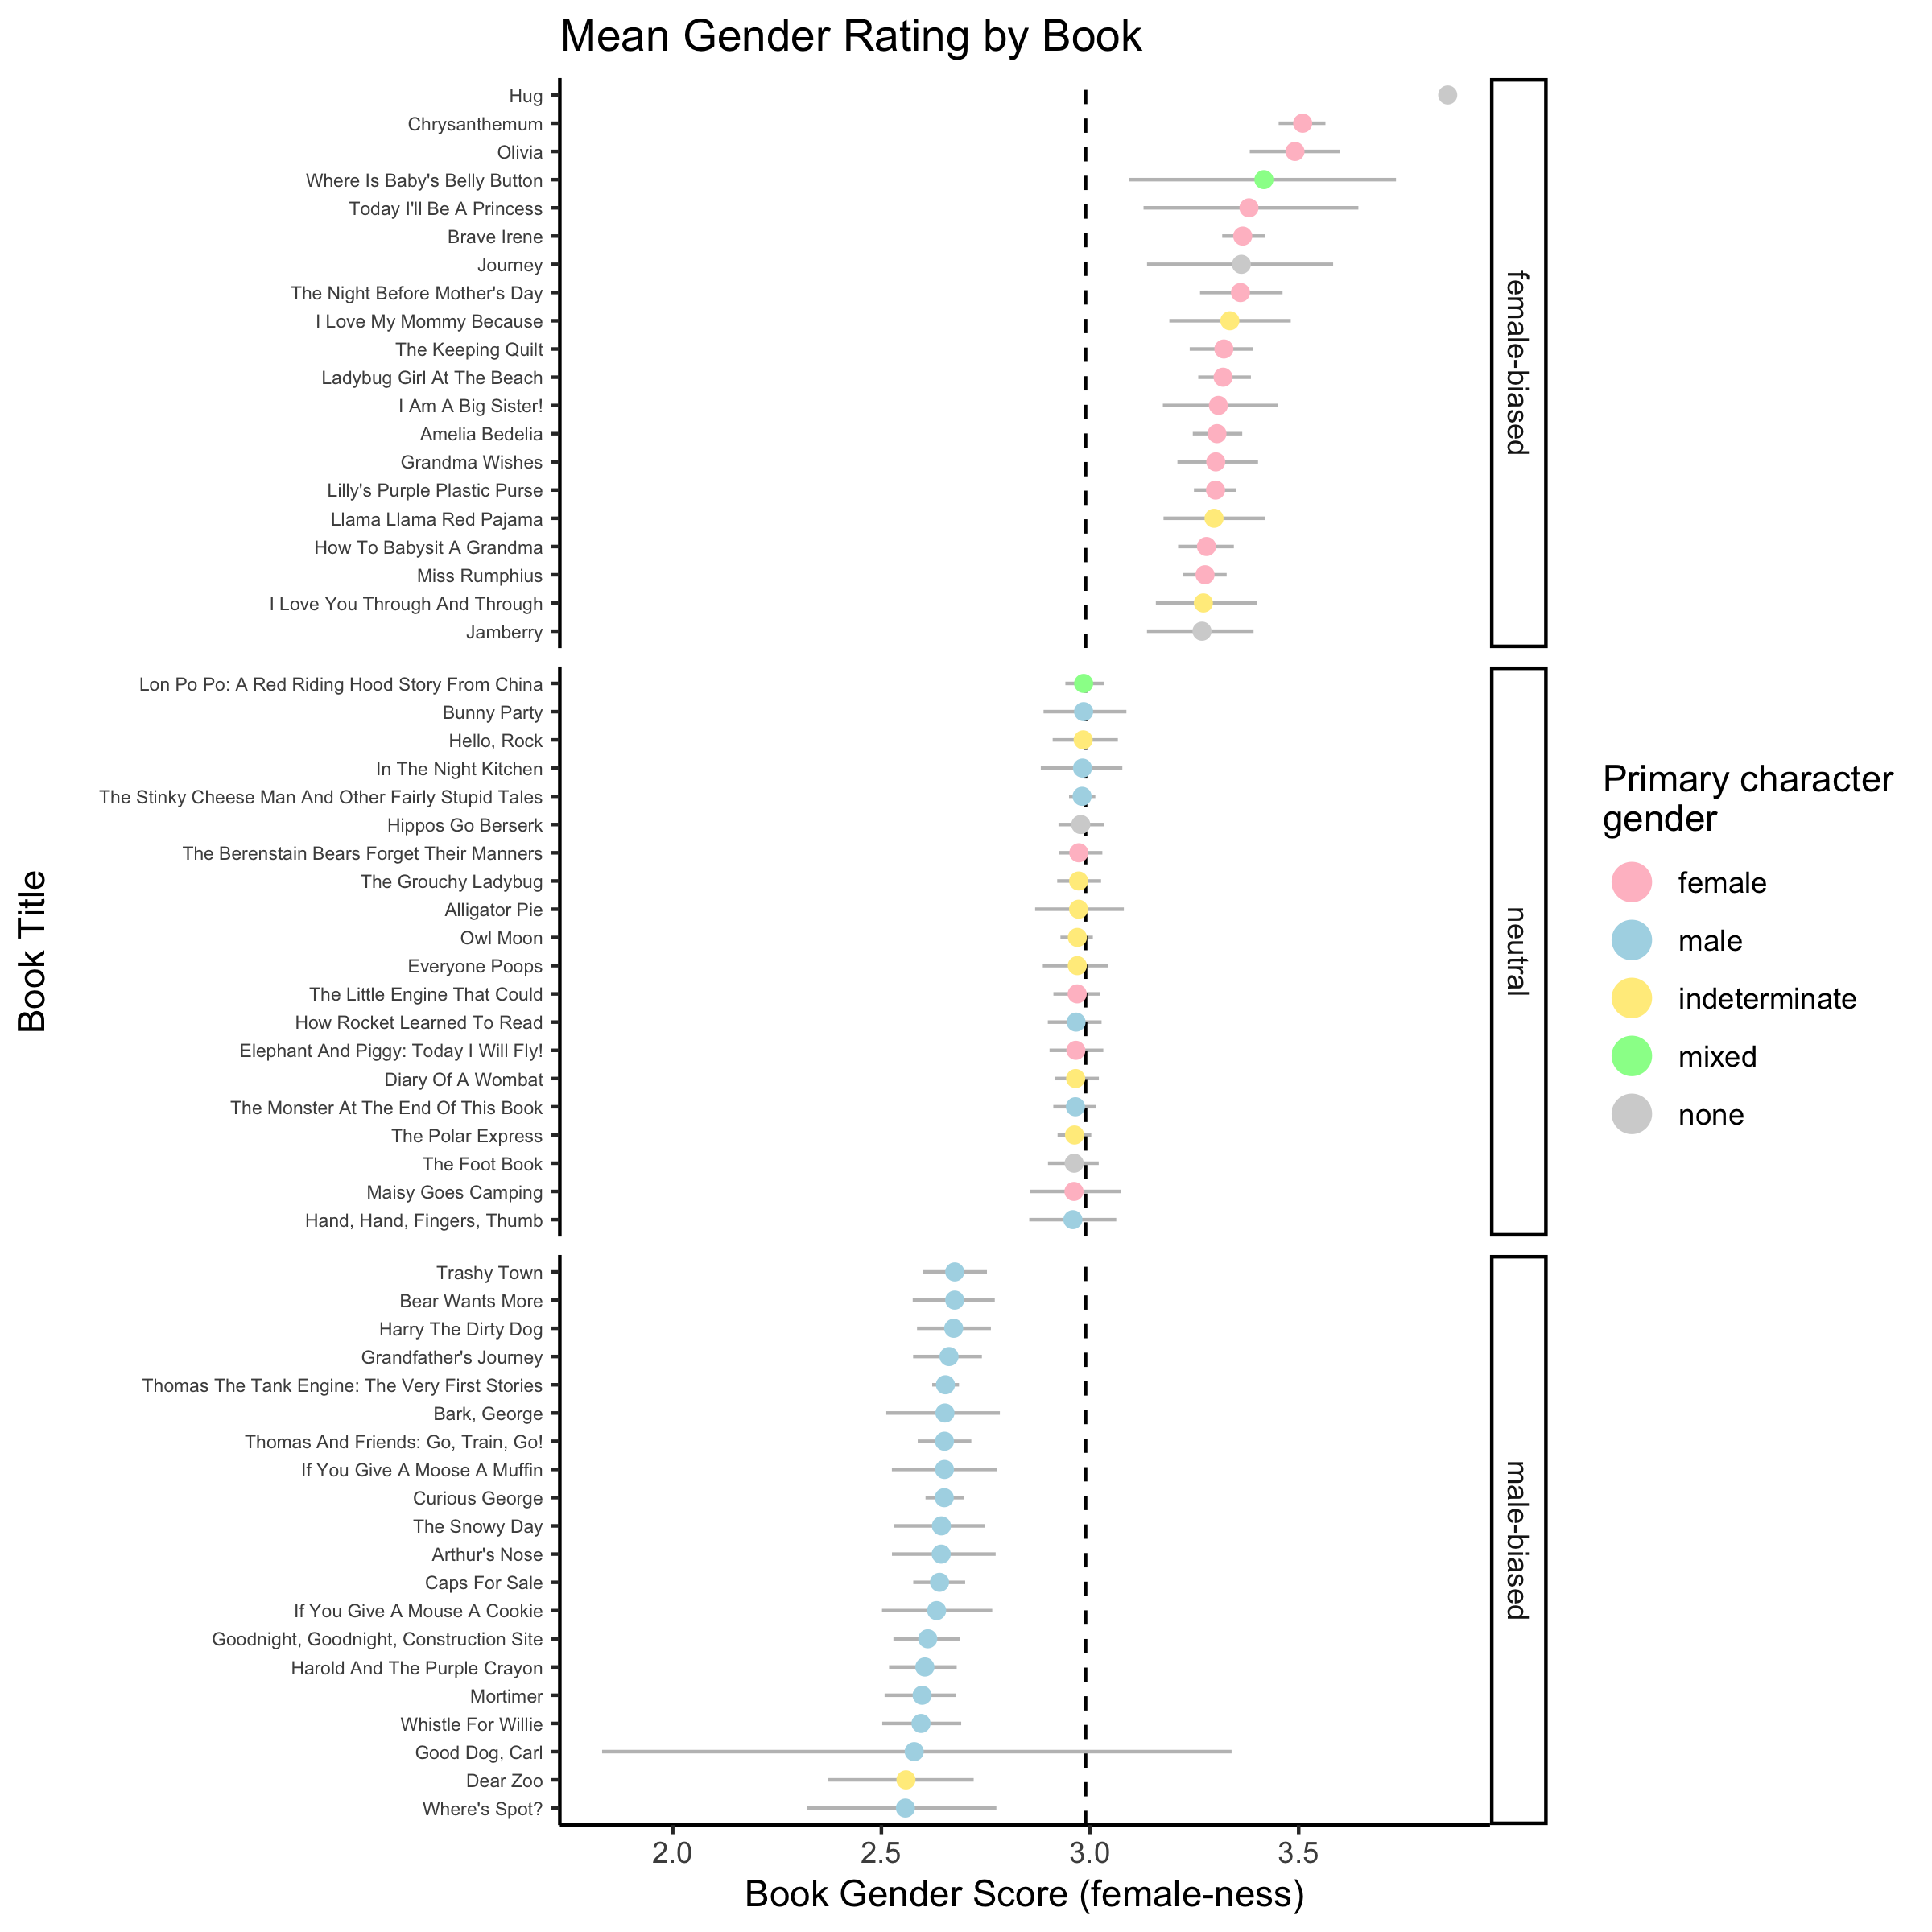
\includegraphics{kidbookgender_psych_sci_files/figure-latex/bookforest-1} \caption{Overall gender rating of  a subset of books, the 20 with the highest feminine bias scores, the 20 with the highest masculine bias scores, and 20 from the neutral range. Bias scores are calculated from the mean gender ratings of words in each book (tokens). The dashed line indicates the overall mean across books, and color indicates the gender of the primary character. Ranges are bootstrapped 95\% CIs.}\label{fig:bookforest}
\end{figure}

\begin{figure}[t!]
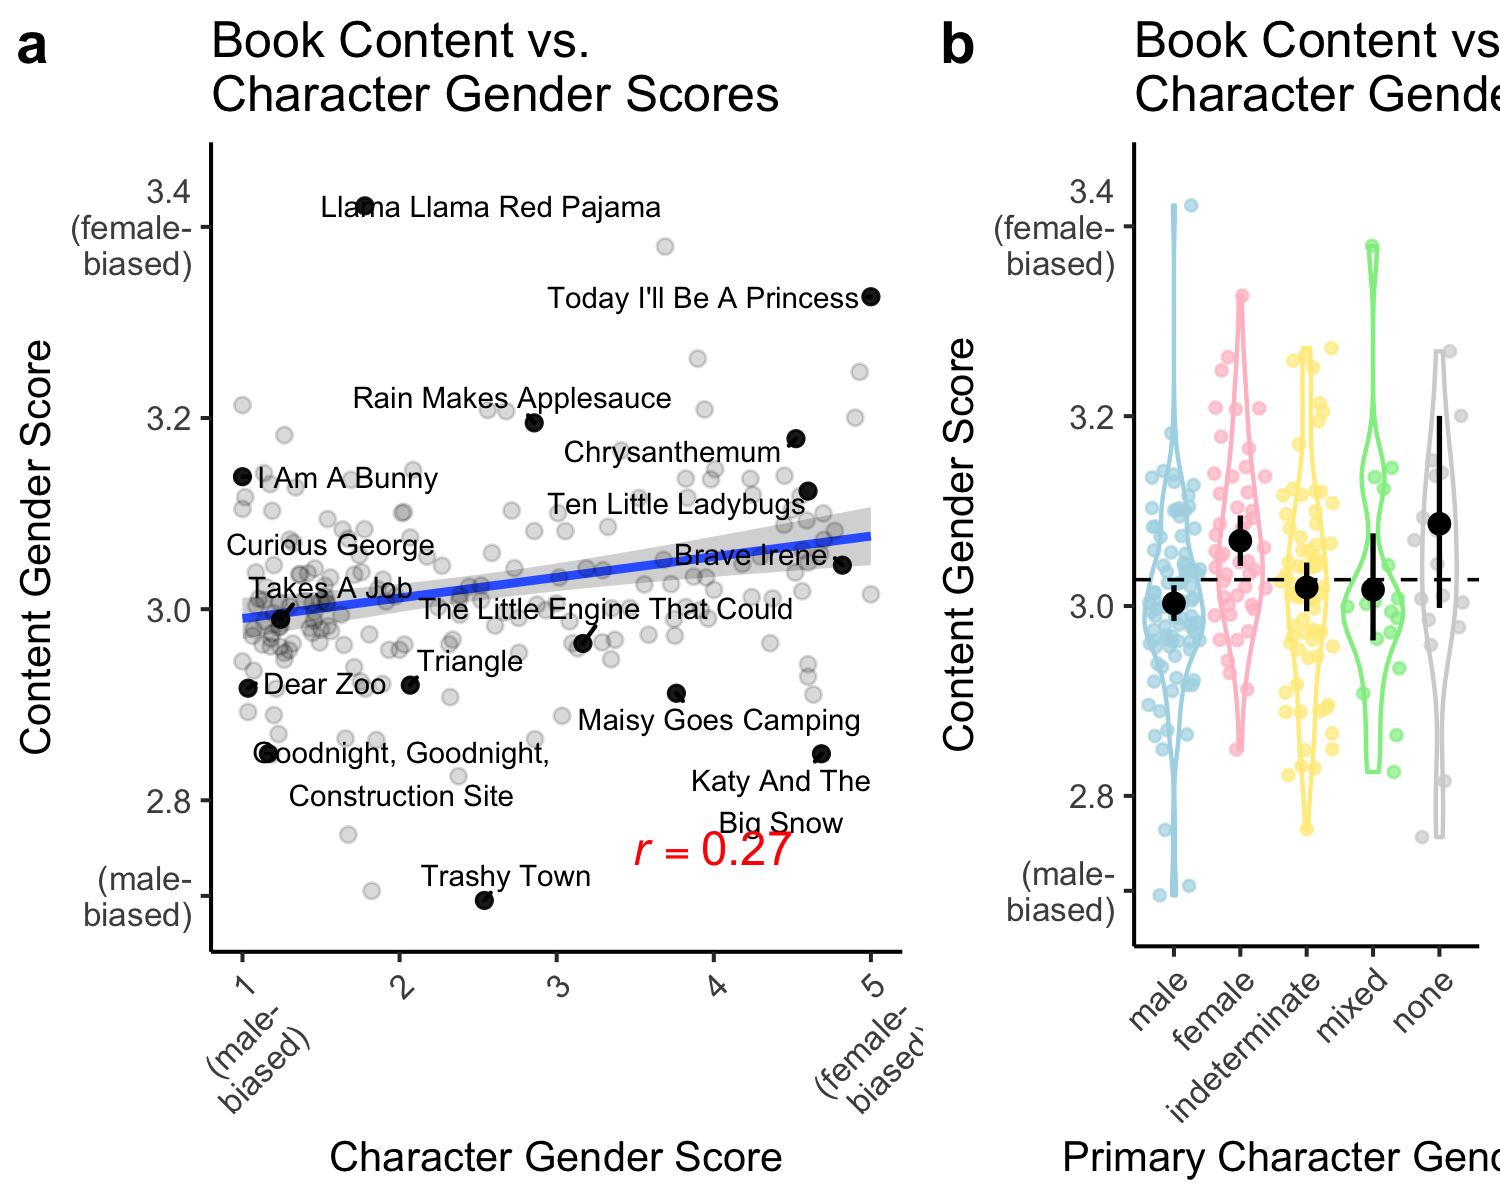
\includegraphics[width=\textwidth,]{kidbookgender_psych_sci_files/figure-latex/characterplot-1} \caption{(a) Mean content gender score for each book as a function of mean character gender score. Higher values indicate a greater propensity for female-biased words. Error bar shows the standard error of the linear model fit. (b) Distribution across books of content gender score as a function of primary character gender. Colored points show individuals books (one point excluded for visibility). Dashed line shows content gender score grand mean. Black points and ranges show mean and bootstrapped 95\% percent confidence intervals for books of each primary character gender type.}\label{fig:characterplot}
\end{figure}

Differences in overall gender bias may be due to the distribution of content words without \enquote{intrinsic} gender (e.g., \emph{beautiful}, \emph{fight}) but also to differences in the occurrence of intrinsically gendered words such as names (\emph{Jill}), pronouns (\emph{her}), and relational/generic gender terms (e.g., \emph{mom}, \emph{lady}). We therefore calculated two additional bias measures, one including only the intrinsically-biased words (the character gender score) and the other including all words except the intrinsically-biased ones (the content gender score). Both the character (\emph{M} = 2.53 {[}2.36, 2.69{]}; \emph{r} = 0.76 {[}0.7, 0.82{]}, \emph{p} \textless{} .001) and content scores (\emph{M} = 3.03 {[}3.01, 3.04{]}; \emph{r} = 0.7 {[}0.63, 0.76{]}, \emph{p} \textless{} .001) were correlated with the overall gender score. Thus, both gendered content words and intrinsically gendered words contribute to the overall gender differences between books.

Character and content scores had a moderate positive correlation with each other (\emph{r} = 0.27 {[}0.13, 0.4{]}, \emph{p} \textless{} .001). Books with more feminine-biased (less masculine-biased) content words do tend to have more female names, pronouns and other intrinsically gendered words (\autoref{fig:characterplot}a). This finding suggests that gender biases reported by adults for content words are potentially inferable from the character associations of the content words in the book texts.

Whereas the character gender score above reflects the extent to which males and females are mentioned in a book, the gender of the story protagonist may be particularly influential for children. For each book, we manually coded the name of the primary protagonist character(s) and the character's gender as determined from the text (i.e., not based on the illustrations). A character was considered a protagonist if that character was the primary agent of the story, even if in a collaborative fashion with another protagonist. The main character(s) were classified as either female, male, mixed, or indeterminate (Wagner, 2017). A book was coded as \enquote{mixed} if there was more than one primary character, and their gender composition was heterogeneous, and as \enquote{indeterminate} if a given primary character had a gender that could not be determined from the text. Two research assistants and the second author coded character gender. Coders agreed on the protagonist type for 97\% of books. Discrepancies were resolved through discussion.

About half of the books (142/248; 57\%) had gendered primary characters that were exclusively male or exclusively female. Two-thirds of these books had male primary characters (\emph{N} = 94; \(\chi^2\); \emph{d} = 0.68 {[}0.34, 1.03{]}). Of the remaining books, 69 (28\%) had main characters(s) of indeterminate gender, 17 (7\%) had main characters of mixed genders, and 20 (8\%) had no main character(s). We then examined book genderedness as a function of the gender of the primary character, using both content and character scores. Books with female primary characters tended to have higher female content scores (\emph{M} = 3.07 {[}3.04, 3.1{]}; \emph{t}(47) = 2.96, \emph{p} = 0.005; \emph{d} = 0.43 {[}0.14, 0.73{]}), compared to the overall averages, whereas books with male primary characters tended to have relatively higher male content scores (\emph{M} = 3 {[}2.98, 3.02{]}; \emph{t}(93) = -2.52, \emph{p} = 0.01; \emph{d} = -0.26 {[}-0.48, -0.06{]}; \autoref{fig:characterplot}b). Notably, however, there was a large degree of variability in content scores across books of a given gender (female: \(SD\) = 0.72; male: \(SD\) = 0.69), suggesting that while some books contain gender stereotypes, others do not.

Our findings suggest that books vary appreciably along the dimension of gender in terms of both their content and characters. The gender distribution of characters we observe is comparable to that reported previously in a smaller sample of books (Wagner, 2017). Together, the gender character and gender content data provide converging evidence that information about gender associates of content words is present in the text of children's books: Books with female characters tend to have content stereotypically associated with females, whereas books with male characters tend to have content stereotypically associated with males.

\hypertarget{study-1c-validation-of-book-gender-bias-measure}{%
\subsection{Study 1c: Validation of book gender bias measure}\label{study-1c-validation-of-book-gender-bias-measure}}

One potential limitation of our method in Study 1b for estimating book bias is that the text in each book is treated as a \enquote{bag of words} --- a simple average of the gender bias of all the words occurring in a book. If book text contains frequent instances in which stereotype-relevant information is conveyed by relying on sentence syntax, our method may not accurately reflect gender stereotypes. For example, a book that contains the sentence \enquote{Sally is brave} and \enquote{Sally is not brave} would result in similar gender bias estimates under the measure used in Study 1b. In Study 1c, we validate the book stereotype measure used in Study 1b by asking adult participants to characterize the stereotypes conveyed in books on the basis of the complete, raw book text.

\hypertarget{method-2}{%
\subsubsection{Method}\label{method-2}}

Participants (\emph{N} = 152; 81 who identified as female, 65 who identified as male, and 6 who did not provide a response) were recruited on Amazon Mechanical Turk.

We divided the books in our corpus into quintiles based on the gender score described in Study 1b, and selected 15 books each from the first (female-biased: \emph{M} = 3.23; \emph{SD} = 0.06), third (neutral: \emph{M} = 2.96; \emph{SD} = 0.03), and fifth quintiles (\emph{M} = 2.64; \emph{SD} = 0.03) to norm further. We excluded books that were either very short or very long (less than 100 words, or more than 900 words), or did not have a named, gendered main character.

Participants were presented with the complete text of an individual book, and told that they would be asked questions about the characters in the story. After reading the text, participants were asked to list 2-5 main activities of particular character in the story in a free response form (e.g., \enquote{List 2-5 main activities THOMAS does in the story.}). The book text was displayed on the same page that responses were elicited, such that participants did not have to rely on their memory to answer the question. Next, participants were asked to complete a similar procedure but instead provide descriptions of a character, rather than associated activities (e.g., \enquote{List 2-5 words to describe THOMAS does in the story.}). This procedure was repeated for all main and secondary characters in a book. Each participant provided responses for both character activities and character descriptions for a sample of three books.

On average, participants generated 3.83 responses per question (\emph{SD} = 1.24). Participants' responses were lemmatized, corrected for spelling, and, in cases where a multi-word phrase (e.g., \enquote{builds a castle}) was listed, the first word was selected for analysis. We identified the part of speech for the target word and excluded responses of the wrong class, analyzing only words that could be a verb for the activity question and an adjective, adverb, or noun for the description question. We also excluded responses that were very long (more than 35 characters), as these were likely to be full sentences rather than activity or description words. In total, 4\% of responses were excluded, leading to a final sample of 4,889 responses and 947 unique lemmas. We then analyzed the gender bias of the activity and description words using previously-collected human judgments of word gender bias. Combining word judgments from Study 1a and an additional set of norms (see SI), we obtained word gender judgments for all words that were produced more than once across the dataset (93.41\% of all words).

\hypertarget{results-1}{%
\subsubsection{Results}\label{results-1}}

The key question was whether the activities and descriptions of characters, derived by human participants reading the full book text, were gender-biased in a way that was predicted by the gender bias of the book as estimated in Study 1b. We fit a mixed-effect linear regression predicting word gender bias for character activity words with book gender bias (male, female or neutral) as a fixed effect, and book and participant as random intercepts. Participants produced activities that were more female-biased for female-biased books, as compared to male-biased books (\(\beta\) = 0.28; \emph{SE} = 0.09; \emph{t} = 3.08; see SI for full model results). The gender bias of activities for characters in neutral books did not differ from male-biased books (\(\beta\) = 0.04; \emph{SE} = 0.09; \emph{t} = 0.41). In a model predicting the gender bias of character descriptions, descriptions of characters in both neutral (\(\beta\) = 0.34; \emph{SE} = 0.14; \emph{t} = 2.41) and female-biased (\(\beta\) = 0.67; \emph{SE} = 0.14; \emph{t} = 4.87) books were rated as more strongly associated with females, relative to male-biased books. These data suggest that the book gender bias measure described in Study 1b captures aspects of books gender bias, even after taking into account more nuanced information about a book's text.

\hypertarget{study-2-measuring-gender-bias-through-co-occurrence-statistics}{%
\section{Study 2: Measuring gender bias through co-occurrence statistics}\label{study-2-measuring-gender-bias-through-co-occurrence-statistics}}

So far we have presented findings about gendered information in children's books based on adult gender norms and semantic representations derived from adult text. The results are relevant to the beliefs of adults who read books with children, which they may convey in conversation during shared reading. However, we also want to understand what a child may learn about gender from the statistics in children's books alone, independent of other information sources.

We next trained word embedding models on the WCBC to understand what gender biases are present in the texts themselves. We find that the gender bias of words---estimated only from word co-occurrences in the corpus itself---is correlated with adult judgments of gender association. We also find that more specific gender stereotypes are reflected in the book text.

\hypertarget{study-2a-word-gender-associations-in-the-childrens-book-corpus}{%
\subsection{Study 2a: Word gender associations in the Children's Book Corpus}\label{study-2a-word-gender-associations-in-the-childrens-book-corpus}}

\hypertarget{method-and-results-1}{%
\subsubsection{Method and Results}\label{method-and-results-1}}

We estimated the extent to which gender associations were encoded in the language co-occurrence statistics in our corpus by training a word embedding model on the full corpus of text from all 247 books (see SI for training details). We then estimated the gender association for each word by calculating its mean semantic similarity (cosine distance) to a set of female words (\enquote{woman,} \enquote{girl,} \enquote{sister,} \enquote{she,} \enquote{her,} and \enquote{daughter}), and a set of male words (\enquote{man,} \enquote{boy,} \enquote{brother,} \enquote{he,} \enquote{him,} and \enquote{son}). A female gender score was calculated for each word as the mean female similarity minus the mean male similarity. For comparison, we also estimated a female score from models trained on an identically sized corpus of adult fiction published from 1990 to 2017 (Corpus of Contemporary American English; Davies, 2008), and a much larger corpus of Wikipedia (Bojanowski et al., 2016). We then examined how these estimates of word gender bias derived from language statistics compared to the gender norms we had previously collected from participants.

\begin{table}

\caption{\label{tab:wordgendertable}Relationships between word gender biases}
\centering
\fontsize{7}{9}\selectfont
\begin{threeparttable}
\begin{tabular}[t]{lrrr}
\toprule
 & \makecell[l]{Human\\gender\\ratings} & \makecell[l]{Distributed\\semantics\\(WCBC)} & \makecell[l]{Distributed\\semantics\\(COCA)}\\
\midrule
Distributed semantics (WCBC) & 0.27 &  & \\
Distributed semantics (COCA) & 0.39 & 0.36 & \\
Distributed semantics (Wikipedia) & 0.66 & 0.32 & 0.42\\
\bottomrule
\end{tabular}
\begin{tablenotes}[para]
\item \textit{Note:} 
\item Correlation values are Pearson's $r$. All correlations are significant at the $p$ < .001 level. WCBC = model trained on Wisconsin Children’s Book Corpus; COCA = Davies, 2008; Wikipedia = Bojanowski et al., 2016.
\end{tablenotes}
\end{threeparttable}
\end{table}

There were 1,893 words common across the word embedding models and human gender norms dataset. Estimates of gender bias from the WCBC were correlated with our adult judgments of word bias (\emph{r} = 0.27 {[}0.23, 0.31{]}, \emph{p} \textless{} .001). Estimates of gender bias from the WCBC were also correlated with word level gender bias estimates from a model trained on adult fiction (\emph{r} = 0.36 {[}0.32, 0.4{]}, \emph{p} \textless{} .001), as well as the model trained on Wikipedia (\emph{r} = 0.32 {[}0.28, 0.36{]}, \emph{p} \textless{} .001; see \autoref{tab:wordgendertable} for all pairwise correlations). This pattern suggests that the word-level gender biases reported by adults could, at least partially, be learned from the co-occurrence language statistics in the WCBC.

\hypertarget{study-2b-specific-gender-biases-in-the-childrens-book-corpus}{%
\subsection{Study 2b: Specific gender biases in the Children's Book Corpus}\label{study-2b-specific-gender-biases-in-the-childrens-book-corpus}}

\hypertarget{method-and-results-2}{%
\subsubsection{Method and Results}\label{method-and-results-2}}

Next, we asked whether specific gender stereotypes, beyond individual word biases, are also present in the statistics of children's books. We focused in particular on four gender stereotypes that have been demonstrated in adults and children in the social psychology literature: (1) Women as \enquote{good}, men as \enquote{bad}; (2) Women as better at language skills, men as better at math skills; (3) Women as better at art skills, men as better at math skills, and (4) Women as family-oriented, men as career-oriented. Each of these stereotypes has been demonstrated behaviorally in prior work through both explicit measures (e.g., asking \enquote{How strongly do you associate career and family with males and females?}) and implicit measures, such as the Implicit Association Test (IAT; Greenwald, McGhee, and Schwartz, 1998; \autoref{tab:iattable}). The IAT quantifies these associations using reaction time in a word categorization task (e.g., women-good/men-bad vs.~women-bad/men-good), though not without criticism about its validity (Greenwald et al., 2020; Oswald, Mitchell, Blanton, Jaccard, \& Tetlock, 2013). Faster responses in this task are taken to indicate that two categories are more closely cognitively associated.

Previous work has shown that the same biases demonstrated in the IAT are also present in the distributional semantics of language (Caliskan, Bryson, \& Narayanan, 2017; Lewis \& Lupyan, 2020). A bias can be quantified in a word embedding model as an effect size, using the same set of word items as in the behavioral IAT. The effect size is calculated as the relative (cosine) similarity of male words (e.g., \enquote{men}) to male-stereotyped words (e.g., \enquote{work}), compared to the relative similarity of female words (e.g., \enquote{women}) to female-stereotyped words (e.g., \enquote{family}; see SI for formal effect size description). Stereotypes that are revealed in the IAT as measured through reaction time (e.g., men-work; women-family) tend to be reflected in word embedding models, as measured by cosine distance.

\begingroup\fontsize{9}{11}\selectfont

\begin{ThreePartTable}
\begin{TableNotes}[para]
\item \textit{Note:} 
\item The left column describes the bias; the middle column lists the actual words tested for the target categories; the right column cites behavioral studies measuring the psychological bias. The words for the ``female" and ``male" categories were identical across all tests (see Main Text). Note that the words differ slightly from the stimuli used in the behavioral studies. ``C" and ``A" in citations indicate whether  participants were children or adults, respectively.
\end{TableNotes}
\begin{longtabu} to \linewidth {>{\raggedright\arraybackslash}p{9em}>{\raggedright\arraybackslash}p{27em}>{\raggedright\arraybackslash}p{15em}}
\caption{\label{tab:iattable}Four IATs used to study gender bias}\\
\toprule
Psychological Bias & Target Words & Behavioral Studies\\
\midrule
women as good;\newline men as bad & ``good": good, happy, gift,  sunshine, heaven\newline ``bad": bad, awful, sick, trouble, hurt & Cveneck, Meltzoff, \& Greenwald (2011b, C); Skowronski \& Lawrence (2001, C/A); Greenwald et al. (2002, A); Rudman \& Goodman (2004, A)\\
\addlinespace\addlinespace
women and family;\newline men and career & ``family": family, parents, children, home, cousins, wedding\newline ``career": job,  work,  money, office, business, desk & Nosek, Banaji,   \& Greenwald (2002, A)\\
\addlinespace\addlinespace
women and language;\newline men and math & ``language": books, read, write, story, letters, spell\newline ``math": numbers, count,  sort,  size, shapes, different & Cveneck, Meltzoff, Greenwald (2011a, C); Nosek, Banaji,  \& Greenwald, (2002, A)\\
\addlinespace\addlinespace
women and arts;\newline  men and math & ``art": art, paint, draw, books, dance, story\newline ``math": numbers, count,  sort,  size, shapes, different & Nosek, Banaji \& Greenwald (2002, A)\\
\bottomrule
\insertTableNotes
\end{longtabu}
\end{ThreePartTable}
\endgroup{}

We used this same method to measure the extent to which gender-related psychological biases were also present in the language statistics of the WCBC. Target category items are listed in \autoref{tab:iattable}, along with citations for the corresponding behavioral IAT experiments with children and adults. Gender category word items were identical to the female score measure above. Other items were taken from the corresponding behavioral experiments, replacing items with more child-friendly alternatives in cases where the target word did not occur in the WCBC (e.g., \enquote{algebra} was changed to \enquote{numbers}). We conducted this analysis on a model trained on the WCBC, as well as models trained on a sample of the adult fiction section of COCA matched in size to the WCBC (Davies, 2008) and a model trained on Wikipedia (Bojanowski et al., 2016). The starting point for the text from the adult fiction book was randomly determined. We trained 10 models each on the COCA and WCBC corpora and estimated the average effect size for each IAT type.

\begin{figure}[t!]
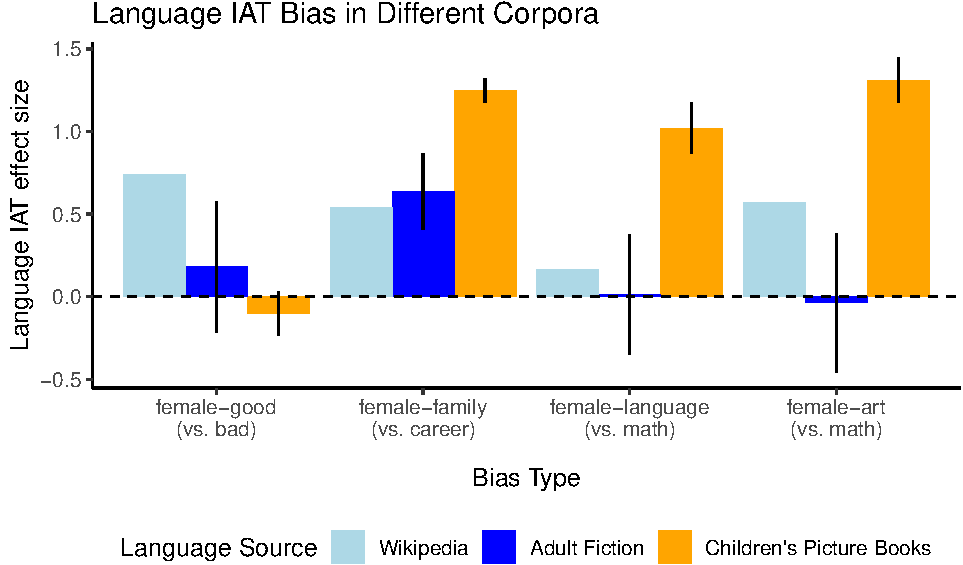
\includegraphics[width=\textwidth,]{kidbookgender_psych_sci_files/figure-latex/languageiat-1} \caption{Estimates of the magnitude of gender biases in word embedding models trained on the Wisconsin Children’s Book Corpus (orange), adult fiction corpus (COCA; dark blue), and Wikipedia (light blue). Positive effect sizes indicate a bias to associate women with the stereotypical category (e.g., ‘family'); negative effect sizes indicate a bias to associate women with the non-stereotypical category (e.g., ‘career’).  Ranges indicate 95\% confidence intervals across models. Biases are described more fully in Table 3.}\label{fig:languageiat}
\end{figure}

\autoref{fig:languageiat} shows the effect size for each of the four biases from models trained on each of the three corpora types. Positive values indicate a bias to associate women with the stereotypical female category (e.g.~women-family). Three of the four gender biases were present in the co-occurrence statistics of the WCBC -- Language-Math, Arts-Math, and Family-Career. Importantly, these biases were larger in children's books than in corpora containing mostly adult-directed language. This finding that behaviorally measurable gender biases are present in an exaggerated form in books for young children provides additional evidence that these books instantiate gender stereotypes that may influence children's learning of gender stereotypes.

In summary, in Study 2, we that adult word gender associations and specific gender biases that have been demonstrated behaviorally in adults and children, such as the bias to associate girls with language and boys with math, are both reflected in the co-occurrence statistics of the children's book corpus.

\hypertarget{study-3-book-gender-and-child-gender}{%
\section{Study 3: Book Gender and Child Gender}\label{study-3-book-gender-and-child-gender}}

The results so far suggest that the text of popular children's books contains rich information about gender. In this final study, we sought to begin to understand the processes through which this information might influence children's socialization into gender stereotypes by examining who is being exposed to these books. We created a novel measure based on the content of book reviews on a large online bookstore and validated this measure using existing survey data directly measuring the audience of a book. These data indicate that children's books more frequently read to girls tend to have both more female content and more female characters, and children's books more frequently read to boys tend to have both more male content and more male characters.

\hypertarget{method-3}{%
\subsubsection{Method}\label{method-3}}

For each book in the WCBC we collected a sample of the most recent reviews on Amazon.com. There were reviews for all but two books, with an average of 473.96 reviews per book (\emph{SD} = 194.53; min = 1; max = 1,290). The content of each review was coded for the presence of 16 gendered kinship terms (e.g., \enquote{son}, \enquote{daughter}, \enquote{nephew}, \enquote{niece}; see SI for full list). We selected these target words because they had a high likelihood of referring to the child for whom the book was purchased (e.g., \enquote{My son loves \emph{Goodnight Moon}.}), rather than referring to a book character. All but two books had reviews containing at least one of our target gendered kinship terms. Overall, 27.63\% of reviews per book contained at least one target gendered kinship term (\emph{SD} = 0.08). For each review, we calculated an audience gender score as the proportion of female kinship terms (tokens) present relative to all target kinship words, and then averaged across reviews from the same book to get a book-level estimate of the gender of book addressees (\emph{M} = 0.49; \emph{SD} = 0.19; see SI for supplemental models predicting book gender at the review level).

We validated our computed audience gender score by comparing it to survey data collected by Hudson Kam \& Matthewson (2017), who asked a sample of 1,107 Canadian caregivers to list the five books most frequently read to their male or female child. Of the books with at least 5 survey responses, 103 were also in the WCBC. Our review-based gender measure was positively correlated with Kam and Matthewson's survey based measure (\emph{r} = 0.58 {[}0.44, 0.7{]}, \emph{p} \textless{} .001), suggesting that book reviews can be used to estimate whether a given book is primarily read to boys or girls.

\hypertarget{results-2}{%
\subsubsection{Results}\label{results-2}}

We compared our audience gender score for each book to the measures of book genderedness described above. Both the content gender scores (\emph{r} = 0.37 {[}0.26, 0.48{]}, \emph{p} \textless{} .001) and book character gender scores (\emph{r} = 0.53 {[}0.41, 0.62{]}, \emph{p} \textless{} .001) were correlated with audience gender scores: Books that contained more female-biased content words and more female characters tended to be read more often to girls. In an additive linear model predicting audience gender with both types of gender scores, both content (\(\beta\) = 0.67; \emph{SE} = 0.12; \emph{Z} = 5.47; \emph{p} \textless{} .001) and character gender scores (\(\beta\) = 0.07; \emph{SE} = 0.01; \emph{Z} = 7.32; \emph{p} \textless{} .001) predicted independent, and roughly equal, variance. Together, they accounted for 37\% of the total variance in audience gender.

Consistent with this general pattern, books with female primary characters also tended to be more often read to girls, compared to the overall average (\emph{t}(46) = 7.02, \emph{p} \textless{} .001; \emph{d} = 1.02 {[}0.67, 1.58{]}; \autoref{fig:characterplots}b). Books with male (\emph{t}(92) = -5.12, \emph{p} \textless{} .001; \emph{d} = -0.53 {[}-0.71, -0.35{]}) or gender indeterminate primary characters (\emph{t}(68) = -3.24, \emph{p} = 0.002; \emph{d} = -0.39 {[}-0.59, -0.18{]}) tended to be more often read to boys. Notably, the effect size for girls was more than twice that of boys, suggesting that there was a stronger bias to read books with female content to girls, relative to books with male content to boys. There was no bias in audience gender for books with multiple primary characters of different genders (\emph{t}(16) = 0.24, \emph{p} = 0.81; \emph{d} = 0.06 {[}-0.39, 0.9{]}) or books without primary characters (\emph{t}(19) = -0.56, \emph{p} = 0.58; \emph{d} = -0.13 {[}-0.77, 0.3{]}).

\begin{figure}[t!]
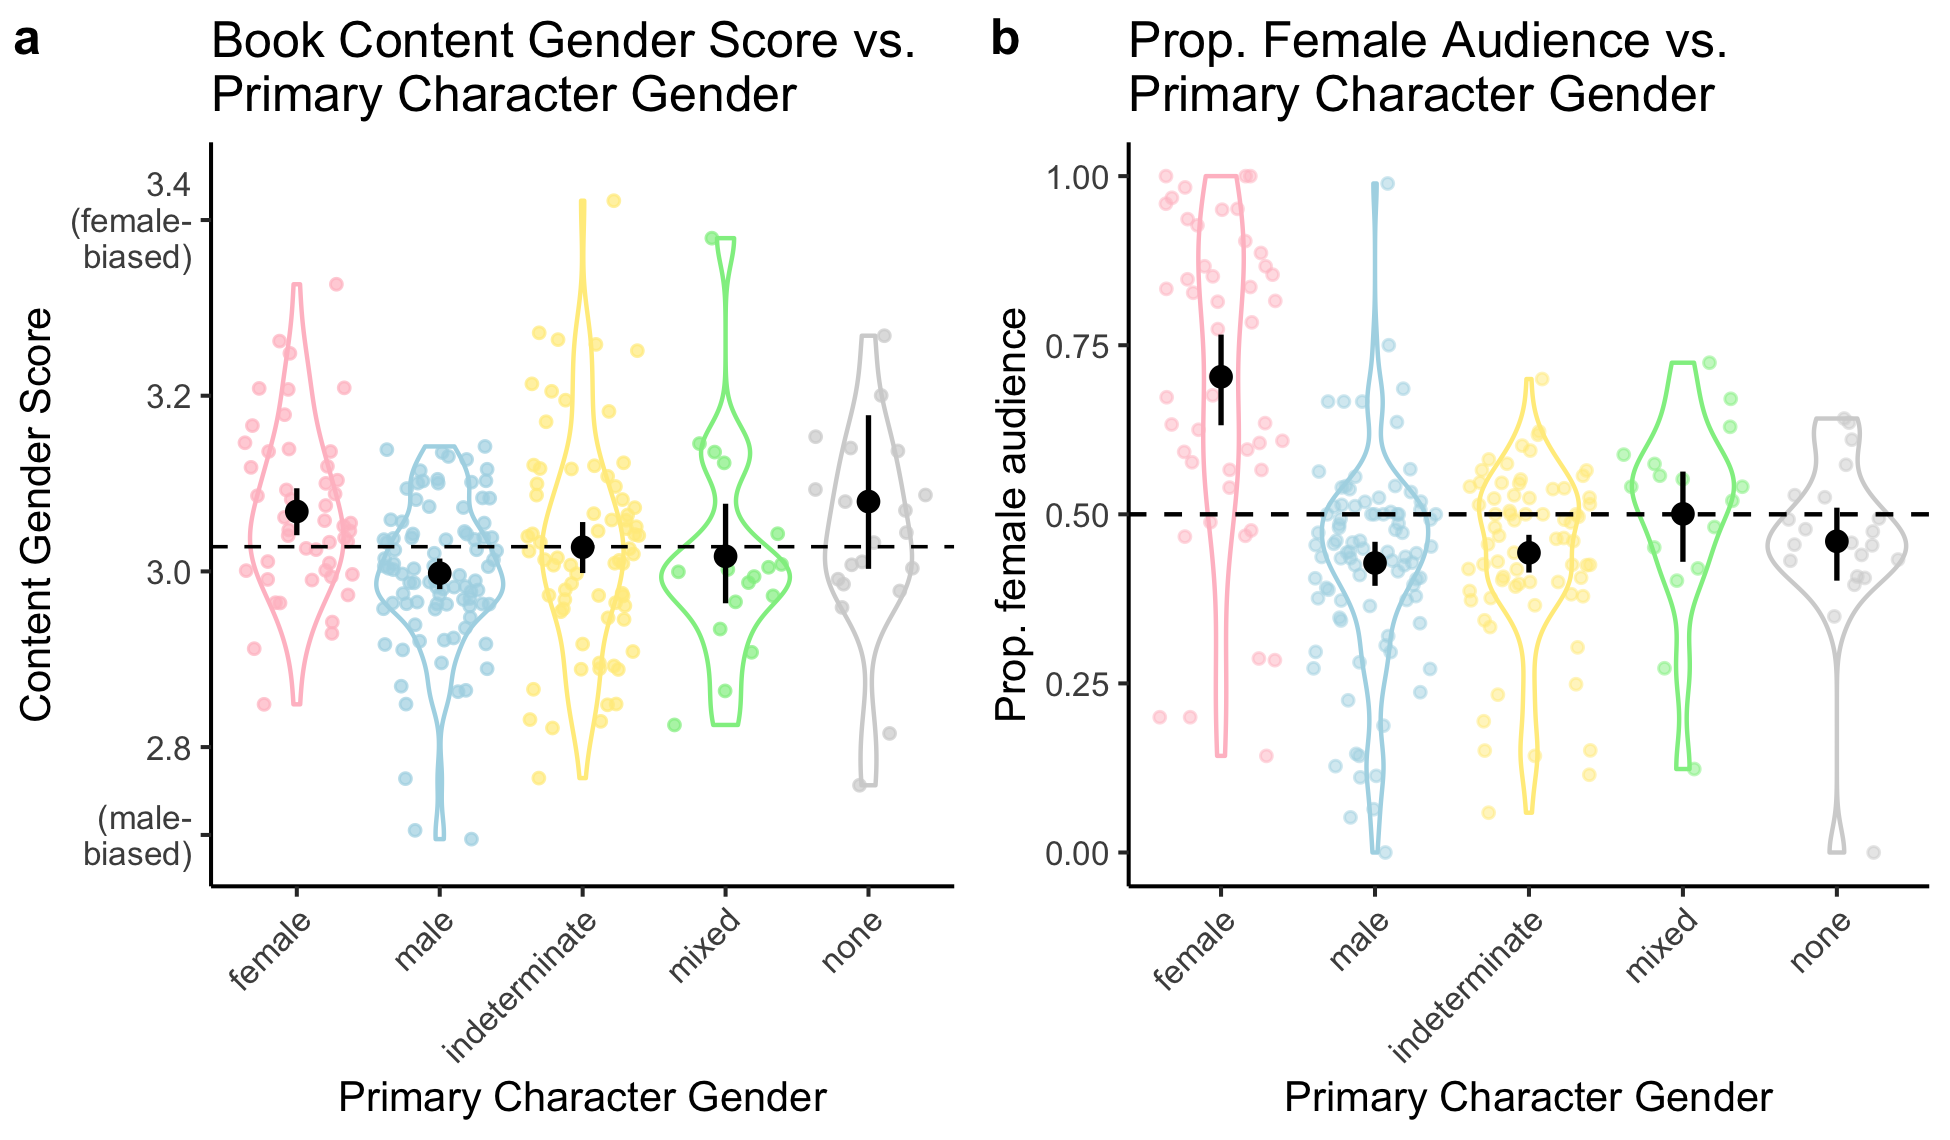
\includegraphics{kidbookgender_psych_sci_files/figure-latex/characterplots-1} \caption{Distribution across books of audience gender as a function of primary character gender. Colored points show individuals books. Dashed line shows grand mean of proportion female audience. Black points and ranges show mean and bootstrapped 95\% percent confidence intervals for books of each primary character gender type.}\label{fig:characterplots}
\end{figure}

In sum, these findings suggest that children's books featuring a particular gender and content associated with that gender tend to be read disproportionately to children of that same gender.

\hypertarget{general-discussion}{%
\section{General Discussion}\label{general-discussion}}

What gender messages are conveyed by popular children's books and who is being exposed to them? We constructed a corpus of 247 contemporary children's books and analyzed the extent to which the books contain gender stereotypes. Using adult judgments of individual words, we found that over half of the words in the corpus tended to be associated with a particular gender. We then used word embedding models to explore the semantic associates of words in the corpus, finding that gender-biased words formed gender stereotypical categories (e.g., social interaction for females; physical interaction for males). Further, word gender biases elicited from adult judgments and more specific gender stereotypes (e.g., boys are relatively better at math, and girls are relatively better at reading) were reflected in the language statistics of the corpus itself, \emph{and} were more exaggerated than in adult fiction. At the book level, we found that books varied in their genderedness, and contained statistical regularities reflecting gender stereotypes (e.g., girl characters tended to do stereotypically girl activities). These statistical regularities were stronger for female stereotypes relative to male stereotypes. Finally, we derived a novel metric for measuring the gender distribution of a book's audience using automated analysis of book reviews. Children tended to be exposed to books that conveyed gender stereotypes about their own gender. Our work provides the first quantitative assessment of the nature of gender messages within contemporary children's books, and reveals that they contain many statistical regularities that could inform children's understanding of gender stereotypes.

There are several reasons to think that the statistical regularities we identified in children's books may be shaping children's gender stereotypes. First, many of the stereotypical patterns that we report are implicit in the distributional statistics of the text, rather than conveyed via explicit statements (\enquote{boys are better at math than girls}). The implicit nature of these messages may make them particularly difficult for adult readers to track or explicitly contradict. Second, children are exposed to books with a caregiver (compared to, e.g., watching TV). The caregiver's presence may signal implicit endorsement of these stereotypes as correct or desirable and lead the child to make to stronger inferences (Lewis \& Frank, 2016; Xu \& Tenenbaum, 2007). Third, our data suggest that children tend to be exposed to books that contain gender stereotypes of their own gender presenting children with more information about own-gender-consistent associations. This may make gender-inconsistent preferences less familiar to children and therefore more difficult to emulate (Bussey \& Bandura, 1999). Filtered through children's cognitive and social biases, children's books may therefore be a potent means of teaching children about gender stereotypes.

Our work characterizes the messages in the text of children's books and begins to address the role they play in socialization, but there are a number of open questions about the causal link between the statistical regularities we observe and the gender stereotypes that children form. Importantly, little is known about how children themselves perceive the messages contained within these books. In the work presented here, we primarily measure word gender bias via adult judgments, yet children do not have the extensive knowledge and experience that underlies adult judgments. The fact that word embedding models trained exclusively on the statistics of the children's book corpus reflect adult-like word gender biases suggests that the adult gender biases could in principle be learned from sources like children's book text, but it is an open question whether they actually do. Future work could more directly address these questions by eliciting child ratings of word gender, and by experimentally manipulating the statistics of children's linguistic input about gender.

An unanswered question from our data is whether the tendency for children to be read books matching their own gender is due to caregiver or child preferences. This question is important in light of recent data on gender development in transgender children (Gülgöz et al., 2019). Transgender children show strong identity with the gender they feel they are by three years of age. If transgender children play an active role in their own socialization (Martin \& Ruble, 2004), our data suggest that children's books could be an early source of gender information for transgender children.

There is no doubt that shared reading has numerous benefits. However, our data show that embedded within contemporary children's books are pervasive gender stereotypes --- indeed stronger than those found in adult-directed literature. Exposure to these language-embedded biases may lead to beliefs that help entrench gender disparities. Our work suggests caregivers may be able to influence children's gender stereotype development through their choices in which books to read to their children.

\newpage

\hypertarget{references}{%
\section{References}\label{references}}

\setlength{\parindent}{-0.5in}
\setlength{\leftskip}{0.5in}

\hypertarget{refs}{}
\leavevmode\hypertarget{ref-bian2017gender}{}%
Bian, L., Leslie, S.-J., \& Cimpian, A. (2017). Gender stereotypes about intellectual ability emerge early and influence children's interests. \emph{Science}, \emph{355}(6323), 389--391.

\leavevmode\hypertarget{ref-bojanowski2016enriching}{}%
Bojanowski, P., Grave, E., Joulin, A., \& Mikolov, T. (2016). Enriching word vectors with subword information. \emph{arXiv Preprint arXiv:1607.01759}.

\leavevmode\hypertarget{ref-bus1995joint}{}%
Bus, A. G., Van Ijzendoorn, M. H., \& Pellegrini, A. D. (1995). Joint book reading makes for success in learning to read: A meta-analysis on intergenerational transmission of literacy. \emph{Review of Educational Research}, \emph{65}(1), 1--21.

\leavevmode\hypertarget{ref-bussey1999social}{}%
Bussey, K., \& Bandura, A. (1999). Social cognitive theory of gender development and differentiation. \emph{Psychological Review}, \emph{106}(4), 676.

\leavevmode\hypertarget{ref-caliskan2017semantics}{}%
Caliskan, A., Bryson, J. J., \& Narayanan, A. (2017). Semantics derived automatically from language corpora contain human-like biases. \emph{Science}, \emph{356}(6334), 183--186.

\leavevmode\hypertarget{ref-chen2017evaluating}{}%
Chen, D., Peterson, J. C., \& Griffiths, T. L. (2017). Evaluating vector-space models of analogy. \emph{arXiv Preprint arXiv:1705.04416}.

\leavevmode\hypertarget{ref-chick2002impact}{}%
Chick, K. A., Heilman-Houser, R. A., \& Hunter, M. W. (2002). The impact of child care on gender role development and gender stereotypes. \emph{Early Childhood Education Journal}, \emph{29}(3), 149--154.

\leavevmode\hypertarget{ref-cimpian2011generic}{}%
Cimpian, A., \& Markman, E. M. (2011). The generic/nongeneric distinction influences how children interpret new information about social others. \emph{Child Development}, \emph{82}(2), 471--492.

\leavevmode\hypertarget{ref-cvencek2011measuring}{}%
Cvencek, D., Greenwald, A. G., \& Meltzoff, A. N. (2011a). Measuring implicit attitudes of 4-year-olds: The Preschool Implicit Association Test. \emph{Journal of Experimental Child Psychology}, \emph{109}(2), 187--200.

\leavevmode\hypertarget{ref-cvencek2011math}{}%
Cvencek, D., Meltzoff, A. N., \& Greenwald, A. G. (2011b). Math--gender stereotypes in elementary school children. \emph{Child Development}, \emph{82}(3), 766--779.

\leavevmode\hypertarget{ref-time_100_kidbooks}{}%
D'Addario, Daniel, Nathan, G., \& Rayman, N. (n.d.). The 100 best children's books of all time. Retrieved from \url{http://time.com/100-best-childrens-books/}

\leavevmode\hypertarget{ref-davies2008corpus}{}%
Davies, M. (2008). The Corpus of Contemporary American English: 450 million words, 1990-present. \emph{https://www.english-Corpora.org/Coca/}.

\leavevmode\hypertarget{ref-diekman2004learning}{}%
Diekman, A. B., \& Murnen, S. K. (2004). Learning to be little women and little men: The inequitable gender equality of nonsexist children's literature. \emph{Sex Roles}, \emph{50}(5-6), 373--385.

\leavevmode\hypertarget{ref-duursma2008reading}{}%
Duursma, E., Augustyn, M., \& Zuckerman, B. (2008). Reading aloud to children: The evidence. \emph{Archives of Disease in Childhood}, \emph{93}(7), 554--557.

\leavevmode\hypertarget{ref-gelman2000gender}{}%
Gelman, S. A., \& Taylor, M. G. (2000). Gender essentialism in cognitive development. \emph{Toward a Feminist Developmental Psychology}, 169--190.

\leavevmode\hypertarget{ref-greenwald2002unified}{}%
Greenwald, A. G., Banaji, M. R., Rudman, L. A., Farnham, S. D., Nosek, B. A., \& Mellott, D. S. (2002). A unified theory of implicit attitudes, stereotypes, self-esteem, and self-concept. \emph{Psychological Review}, \emph{109}(1), 3--25.

\leavevmode\hypertarget{ref-greenwald2020}{}%
Greenwald, A. G., Brendl, M., Cai, H., Cvencek, D., Dovidio, J. F., Friese, M., \ldots{} al. (2020, April). The implicit association test at age 20: What is known and what is not known about implicit bias. PsyArXiv. doi:\href{https://doi.org/10.31234/osf.io/bf97c}{10.31234/osf.io/bf97c}

\leavevmode\hypertarget{ref-gulgoz2019similarity}{}%
Gülgöz, S., Glazier, J. J., Enright, E. A., Alonso, D. J., Durwood, L. J., Fast, A. A., \ldots{} others. (2019). Similarity in transgender and cisgender children's gender development. \emph{Proceedings of the National Academy of Sciences}, \emph{116}(49), 24480--24485.

\leavevmode\hypertarget{ref-high2014literacy}{}%
High, P. C., \& Klass, P. (2014). Literacy promotion: An essential component of primary care pediatric practice. \emph{Pediatrics}, \emph{134}(2), 404--409.

\leavevmode\hypertarget{ref-hill2015simlex}{}%
Hill, F., Reichart, R., \& Korhonen, A. (2015). Simlex-999: Evaluating semantic models with (genuine) similarity estimation. \emph{Computational Linguistics}, \emph{41}(4), 665--695.

\leavevmode\hypertarget{ref-hilliard2010differing}{}%
Hilliard, L. J., \& Liben, L. S. (2010). Differing levels of gender salience in preschool classrooms: Effects on children's gender attitudes and intergroup bias. \emph{Child Development}, \emph{81}(6), 1787--1798.

\leavevmode\hypertarget{ref-kam_2017}{}%
Hudson Kam, C. L., \& Matthewson, L. (2017). Introducing the Infant Bookreading Database (IBDb). \emph{Journal of Child Language}, \emph{44}(6), 1289--1308.

\leavevmode\hypertarget{ref-landauer1997solution}{}%
Landauer, T. K., \& Dumais, S. T. (1997). A solution to Plato's problem: The latent semantic analysis theory of acquisition, induction, and representation of knowledge. \emph{Psychological Review}, \emph{104}(2), 211.

\leavevmode\hypertarget{ref-lewis2016understanding}{}%
Lewis, M. L., \& Frank, M. C. (2016). Understanding the effect of social context on learning: A replication of Xu and Tenenbaum (2007b). \emph{Journal of Experimental Psychology: General}, \emph{145}(9), e72--e80.

\leavevmode\hypertarget{ref-lewis2020}{}%
Lewis, M., \& Lupyan, G. (2020). Gender stereotypes are reflected in the distributional structure of 25 languages. \emph{Nature Human Behaviour}, 1--8.

\leavevmode\hypertarget{ref-maaten2008visualizing}{}%
Maaten, L. van der, \& Hinton, G. (2008). Visualizing data using t-sne. \emph{Journal of Machine Learning Research}, \emph{9}(Nov), 2579--2605.

\leavevmode\hypertarget{ref-martin2004children}{}%
Martin, C. L., \& Ruble, D. (2004). Children's search for gender cues: Cognitive perspectives on gender development. \emph{Current Directions in Psychological Science}, \emph{13}(2), 67--70.

\leavevmode\hypertarget{ref-mikolov2013efficient}{}%
Mikolov, T., Chen, K., Corrado, G., \& Dean, J. (2013). Efficient estimation of word representations in vector space. \emph{arXiv Preprint arXiv:1301.3781}.

\leavevmode\hypertarget{ref-montag2015words}{}%
Montag, J. L., Jones, M. N., \& Smith, L. B. (2015). The words children hear: Picture books and the statistics for language learning. \emph{Psychological Science}, \emph{26}(9), 1489--1496.

\leavevmode\hypertarget{ref-nosek2002harvesting}{}%
Nosek, B. A., Banaji, M. R., \& Greenwald, A. G. (2002). Harvesting implicit group attitudes and beliefs from a demonstration web site. \emph{Group Dynamics: Theory, Research, and Practice}, \emph{6}(1), 101.

\leavevmode\hypertarget{ref-oswald2013predicting}{}%
Oswald, F. L., Mitchell, G., Blanton, H., Jaccard, J., \& Tetlock, P. E. (2013). Predicting ethnic and racial discrimination: A meta-analysis of iat criterion studies. \emph{Journal of Personality and Social Psychology}, \emph{105}(2), 171.

\leavevmode\hypertarget{ref-poulin2002men}{}%
Poulin-Dubois, D., Serbin, L. A., Eichstedt, J. A., Sen, M. G., \& Beissel, C. F. (2002). Men don't put on make-up: Toddlers' knowledge of the gender stereotyping of household activities. \emph{Social Development}, \emph{11}(2), 166--181.

\leavevmode\hypertarget{ref-rudman2004gender}{}%
Rudman, L. A., \& Goodwin, S. A. (2004). Gender differences in automatic in-group bias: Why do women like women more than men like men? \emph{Journal of Personality and Social Psychology}, \emph{87}(4), 494.

\leavevmode\hypertarget{ref-scott2019glasgow}{}%
Scott, G. G., Keitel, A., Becirspahic, M., Yao, B., \& Sereno, S. C. (2019). The Glasgow Norms: Ratings of 5,500 words on nine scales. \emph{Behavior Research Methods}, \emph{51}(3), 1258--1270.

\leavevmode\hypertarget{ref-shutts2010social}{}%
Shutts, K., Banaji, M. R., \& Spelke, E. S. (2010). Social categories guide young children's preferences for novel objects. \emph{Developmental Science}, \emph{13}(4), 599--610.

\leavevmode\hypertarget{ref-skowronski2001comparative}{}%
Skowronski, J. J., \& Lawrence, M. A. (2001). A comparative study of the implicit and explicit gender attitudes of children and college students. \emph{Psychology of Women Quarterly}, \emph{25}(2), 155--165.

\leavevmode\hypertarget{ref-snow1998preventing}{}%
Snow, C. E., Burns, M. S., \& Griffin, P. (1998). \emph{Preventing reading difficulties in young children}. National Academies Press.

\leavevmode\hypertarget{ref-wagner2017factors}{}%
Wagner, L. (2017). Factors influencing parents' preferences and parents' perceptions of child preferences of picture books. \emph{Frontiers in Psychology}, \emph{8}, 1448.

\leavevmode\hypertarget{ref-weisgram2014pink}{}%
Weisgram, E. S., Fulcher, M., \& Dinella, L. M. (2014). Pink gives girls permission: Exploring the roles of explicit gender labels and gender-typed colors on preschool children's toy preferences. \emph{Journal of Applied Developmental Psychology}, \emph{35}(5), 401--409.

\leavevmode\hypertarget{ref-xu2007b}{}%
Xu, F., \& Tenenbaum, J. B. (2007). Sensitivity to sampling in Bayesian word learning. \emph{Developmental Science}, \emph{10}(3), 288--297.

\leavevmode\hypertarget{ref-bian2017gender}{}%
Bian, L., Leslie, S.-J., \& Cimpian, A. (2017). Gender stereotypes about intellectual ability emerge early and influence children's interests. \emph{Science}, \emph{355}(6323), 389--391.

\leavevmode\hypertarget{ref-bojanowski2016enriching}{}%
Bojanowski, P., Grave, E., Joulin, A., \& Mikolov, T. (2016). Enriching word vectors with subword information. \emph{arXiv Preprint arXiv:1607.01759}.

\leavevmode\hypertarget{ref-bus1995joint}{}%
Bus, A. G., Van Ijzendoorn, M. H., \& Pellegrini, A. D. (1995). Joint book reading makes for success in learning to read: A meta-analysis on intergenerational transmission of literacy. \emph{Review of Educational Research}, \emph{65}(1), 1--21.

\leavevmode\hypertarget{ref-bussey1999social}{}%
Bussey, K., \& Bandura, A. (1999). Social cognitive theory of gender development and differentiation. \emph{Psychological Review}, \emph{106}(4), 676.

\leavevmode\hypertarget{ref-caliskan2017semantics}{}%
Caliskan, A., Bryson, J. J., \& Narayanan, A. (2017). Semantics derived automatically from language corpora contain human-like biases. \emph{Science}, \emph{356}(6334), 183--186.

\leavevmode\hypertarget{ref-chen2017evaluating}{}%
Chen, D., Peterson, J. C., \& Griffiths, T. L. (2017). Evaluating vector-space models of analogy. \emph{arXiv Preprint arXiv:1705.04416}.

\leavevmode\hypertarget{ref-chick2002impact}{}%
Chick, K. A., Heilman-Houser, R. A., \& Hunter, M. W. (2002). The impact of child care on gender role development and gender stereotypes. \emph{Early Childhood Education Journal}, \emph{29}(3), 149--154.

\leavevmode\hypertarget{ref-cimpian2011generic}{}%
Cimpian, A., \& Markman, E. M. (2011). The generic/nongeneric distinction influences how children interpret new information about social others. \emph{Child Development}, \emph{82}(2), 471--492.

\leavevmode\hypertarget{ref-cvencek2011measuring}{}%
Cvencek, D., Greenwald, A. G., \& Meltzoff, A. N. (2011a). Measuring implicit attitudes of 4-year-olds: The Preschool Implicit Association Test. \emph{Journal of Experimental Child Psychology}, \emph{109}(2), 187--200.

\leavevmode\hypertarget{ref-cvencek2011math}{}%
Cvencek, D., Meltzoff, A. N., \& Greenwald, A. G. (2011b). Math--gender stereotypes in elementary school children. \emph{Child Development}, \emph{82}(3), 766--779.

\leavevmode\hypertarget{ref-time_100_kidbooks}{}%
D'Addario, Daniel, Nathan, G., \& Rayman, N. (n.d.). The 100 best children's books of all time. Retrieved from \url{http://time.com/100-best-childrens-books/}

\leavevmode\hypertarget{ref-davies2008corpus}{}%
Davies, M. (2008). The Corpus of Contemporary American English: 450 million words, 1990-present. \emph{https://www.english-Corpora.org/Coca/}.

\leavevmode\hypertarget{ref-diekman2004learning}{}%
Diekman, A. B., \& Murnen, S. K. (2004). Learning to be little women and little men: The inequitable gender equality of nonsexist children's literature. \emph{Sex Roles}, \emph{50}(5-6), 373--385.

\leavevmode\hypertarget{ref-duursma2008reading}{}%
Duursma, E., Augustyn, M., \& Zuckerman, B. (2008). Reading aloud to children: The evidence. \emph{Archives of Disease in Childhood}, \emph{93}(7), 554--557.

\leavevmode\hypertarget{ref-gelman2000gender}{}%
Gelman, S. A., \& Taylor, M. G. (2000). Gender essentialism in cognitive development. \emph{Toward a Feminist Developmental Psychology}, 169--190.

\leavevmode\hypertarget{ref-greenwald2002unified}{}%
Greenwald, A. G., Banaji, M. R., Rudman, L. A., Farnham, S. D., Nosek, B. A., \& Mellott, D. S. (2002). A unified theory of implicit attitudes, stereotypes, self-esteem, and self-concept. \emph{Psychological Review}, \emph{109}(1), 3--25.

\leavevmode\hypertarget{ref-greenwald2020}{}%
Greenwald, A. G., Brendl, M., Cai, H., Cvencek, D., Dovidio, J. F., Friese, M., \ldots{} al. (2020, April). The implicit association test at age 20: What is known and what is not known about implicit bias. PsyArXiv. doi:\href{https://doi.org/10.31234/osf.io/bf97c}{10.31234/osf.io/bf97c}

\leavevmode\hypertarget{ref-gulgoz2019similarity}{}%
Gülgöz, S., Glazier, J. J., Enright, E. A., Alonso, D. J., Durwood, L. J., Fast, A. A., \ldots{} others. (2019). Similarity in transgender and cisgender children's gender development. \emph{Proceedings of the National Academy of Sciences}, \emph{116}(49), 24480--24485.

\leavevmode\hypertarget{ref-high2014literacy}{}%
High, P. C., \& Klass, P. (2014). Literacy promotion: An essential component of primary care pediatric practice. \emph{Pediatrics}, \emph{134}(2), 404--409.

\leavevmode\hypertarget{ref-hill2015simlex}{}%
Hill, F., Reichart, R., \& Korhonen, A. (2015). Simlex-999: Evaluating semantic models with (genuine) similarity estimation. \emph{Computational Linguistics}, \emph{41}(4), 665--695.

\leavevmode\hypertarget{ref-hilliard2010differing}{}%
Hilliard, L. J., \& Liben, L. S. (2010). Differing levels of gender salience in preschool classrooms: Effects on children's gender attitudes and intergroup bias. \emph{Child Development}, \emph{81}(6), 1787--1798.

\leavevmode\hypertarget{ref-kam_2017}{}%
Hudson Kam, C. L., \& Matthewson, L. (2017). Introducing the Infant Bookreading Database (IBDb). \emph{Journal of Child Language}, \emph{44}(6), 1289--1308.

\leavevmode\hypertarget{ref-landauer1997solution}{}%
Landauer, T. K., \& Dumais, S. T. (1997). A solution to Plato's problem: The latent semantic analysis theory of acquisition, induction, and representation of knowledge. \emph{Psychological Review}, \emph{104}(2), 211.

\leavevmode\hypertarget{ref-lewis2016understanding}{}%
Lewis, M. L., \& Frank, M. C. (2016). Understanding the effect of social context on learning: A replication of Xu and Tenenbaum (2007b). \emph{Journal of Experimental Psychology: General}, \emph{145}(9), e72--e80.

\leavevmode\hypertarget{ref-lewis2020}{}%
Lewis, M., \& Lupyan, G. (2020). Gender stereotypes are reflected in the distributional structure of 25 languages. \emph{Nature Human Behaviour}, 1--8.

\leavevmode\hypertarget{ref-maaten2008visualizing}{}%
Maaten, L. van der, \& Hinton, G. (2008). Visualizing data using t-sne. \emph{Journal of Machine Learning Research}, \emph{9}(Nov), 2579--2605.

\leavevmode\hypertarget{ref-martin2004children}{}%
Martin, C. L., \& Ruble, D. (2004). Children's search for gender cues: Cognitive perspectives on gender development. \emph{Current Directions in Psychological Science}, \emph{13}(2), 67--70.

\leavevmode\hypertarget{ref-mikolov2013efficient}{}%
Mikolov, T., Chen, K., Corrado, G., \& Dean, J. (2013). Efficient estimation of word representations in vector space. \emph{arXiv Preprint arXiv:1301.3781}.

\leavevmode\hypertarget{ref-montag2015words}{}%
Montag, J. L., Jones, M. N., \& Smith, L. B. (2015). The words children hear: Picture books and the statistics for language learning. \emph{Psychological Science}, \emph{26}(9), 1489--1496.

\leavevmode\hypertarget{ref-nosek2002harvesting}{}%
Nosek, B. A., Banaji, M. R., \& Greenwald, A. G. (2002). Harvesting implicit group attitudes and beliefs from a demonstration web site. \emph{Group Dynamics: Theory, Research, and Practice}, \emph{6}(1), 101.

\leavevmode\hypertarget{ref-oswald2013predicting}{}%
Oswald, F. L., Mitchell, G., Blanton, H., Jaccard, J., \& Tetlock, P. E. (2013). Predicting ethnic and racial discrimination: A meta-analysis of iat criterion studies. \emph{Journal of Personality and Social Psychology}, \emph{105}(2), 171.

\leavevmode\hypertarget{ref-poulin2002men}{}%
Poulin-Dubois, D., Serbin, L. A., Eichstedt, J. A., Sen, M. G., \& Beissel, C. F. (2002). Men don't put on make-up: Toddlers' knowledge of the gender stereotyping of household activities. \emph{Social Development}, \emph{11}(2), 166--181.

\leavevmode\hypertarget{ref-rudman2004gender}{}%
Rudman, L. A., \& Goodwin, S. A. (2004). Gender differences in automatic in-group bias: Why do women like women more than men like men? \emph{Journal of Personality and Social Psychology}, \emph{87}(4), 494.

\leavevmode\hypertarget{ref-scott2019glasgow}{}%
Scott, G. G., Keitel, A., Becirspahic, M., Yao, B., \& Sereno, S. C. (2019). The Glasgow Norms: Ratings of 5,500 words on nine scales. \emph{Behavior Research Methods}, \emph{51}(3), 1258--1270.

\leavevmode\hypertarget{ref-shutts2010social}{}%
Shutts, K., Banaji, M. R., \& Spelke, E. S. (2010). Social categories guide young children's preferences for novel objects. \emph{Developmental Science}, \emph{13}(4), 599--610.

\leavevmode\hypertarget{ref-skowronski2001comparative}{}%
Skowronski, J. J., \& Lawrence, M. A. (2001). A comparative study of the implicit and explicit gender attitudes of children and college students. \emph{Psychology of Women Quarterly}, \emph{25}(2), 155--165.

\leavevmode\hypertarget{ref-snow1998preventing}{}%
Snow, C. E., Burns, M. S., \& Griffin, P. (1998). \emph{Preventing reading difficulties in young children}. National Academies Press.

\leavevmode\hypertarget{ref-wagner2017factors}{}%
Wagner, L. (2017). Factors influencing parents' preferences and parents' perceptions of child preferences of picture books. \emph{Frontiers in Psychology}, \emph{8}, 1448.

\leavevmode\hypertarget{ref-weisgram2014pink}{}%
Weisgram, E. S., Fulcher, M., \& Dinella, L. M. (2014). Pink gives girls permission: Exploring the roles of explicit gender labels and gender-typed colors on preschool children's toy preferences. \emph{Journal of Applied Developmental Psychology}, \emph{35}(5), 401--409.

\leavevmode\hypertarget{ref-xu2007b}{}%
Xu, F., \& Tenenbaum, J. B. (2007). Sensitivity to sampling in Bayesian word learning. \emph{Developmental Science}, \emph{10}(3), 288--297.

\end{document}
